% --- To be compiled with XeLaTeX ---
% ---      Encoding: UTF-8        ---

\documentclass[a4paper, oneside, 11pt]{article}

%fontspec package provides a configurable interface for font selection, and allows complex font choices to be named and later reused. It's needed for XeLaTeX
\usepackage[cm-default]{fontspec}

% Unicode support
\usepackage{xunicode}
\usepackage{xltxtra}

% Default words and phrases in Greek (e.g. 'Περίληψη' instead of 'Abstract'). Also contains hyphenation rules for Greek Language
\usepackage{xgreek}

% Mathematical fonts, theorems etc.
\usepackage{amsfonts}
\usepackage{amsmath}
\usepackage{amsthm}

% Default page layout for consuming a larger portion of the page.
\usepackage{fullpage}

% Greek fonts (Computer Modern)
\setmainfont[Mapping=tex-text]{CMU Serif}

% Auxiliary commands
\newcommand{\red}{\leq_{\text{m}}}

\newtheorem{thm}{Θεώρημα}
\newtheorem{lm}[thm]{Λήμμα}
\newtheorem{col}[thm]{Πόρισμα}

\theoremstyle{definition}
\newtheorem{defn}[thm]{Ορισμός}

\newcommand{\ora}{\vec}

\begin{document}

% Auxiliary commands
\newcommand{\HRule}{\rule{\linewidth}{0.5mm}}

\begin{titlepage}
\begin{center}


\includegraphics[width=0.3\textwidth]{../logos/pyrforos.png}
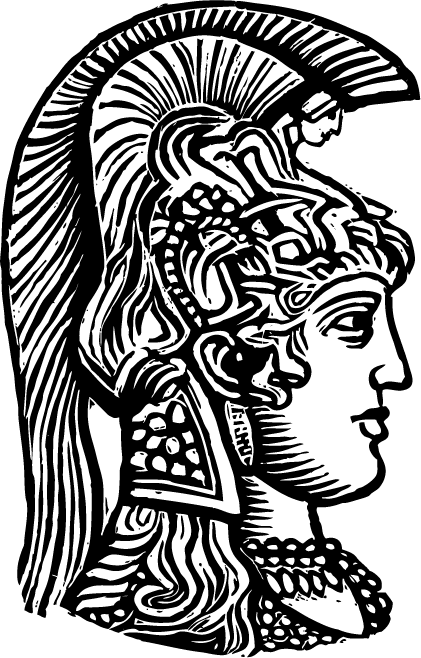
\includegraphics[width=0.2\textwidth]{../logos/uoa.png}\\[1cm]

\textsc{\LARGE Σχολή Ηλεκτρολόγων Μηχανικών και Μηχανικών Υπολογιστών}\\[1.5cm]

\HRule \\[0.4cm]
{\huge \bfseries Υπολογισιμότητα\\
\LARGE Ομάδα Ασκήσεων No. 2}\\[0.4cm]

\HRule \\[1.5cm]

\begin{center}
\textbf{Ομάδα}\\
Αξιώτης Κυριάκος\\
Αρσένης Γεράσιμος
\end{center}

\vfill

{\large \today}
\end{center}

\end{titlepage}


\section*{Άσκηση 1}
Έστω ότι ισχύουν οι 3 συνθήκες της εκφώνησης. Έστω $M_2$ απαριθμητής των πεπερασμένων γλωσσών στο $P$. Θα κατασκευάσουμε μία μηχανή Turing $M_1$ η οποία
με είσοδο $\langle M\rangle$, αν $\langle M\rangle\in P$ θα αποδέχεται σε πεπερασμένο χρόνο. Η $M_1$ απαριθμεί όλα τα ζευγάρια
$(i,j)\in \mathbb{N}^2$ και, για το καθένα, προσομοιώνει τον απαριθμητή $M_2$ για $i$ βήματα. Αν αυτός ο απαριθμητής εμφανίσει τουλάχιστον μία
πεπερασμένη γλώσσα επιλέγουμε την τελευταία που εμφανίστηκε, και έστω ότι αυτή είναι η $L$. Αν ο απαριθμητής δεν εμφανίσει καμία γλώσσα προχωράμε στο
επόμενο ζευγάρι $(i,j)$. Στη συνέχεια, η $M_1$ προσομοιώνει την $M$ με είσοδο κάθε λέξη της $L$, για $j$ βήματα την κάθε μία. Αν η $M$ τις αποδεχθεί
όλες, τότε η $M_1$ αποδέχεται. Διαφορετικά, προχωράει στο επόμενο ζευγάρι $(i,j)$.

Θα δείξουμε ότι η $M_1$ αποδέχεται αν και μόνο αν $L(M)\in P$. Λόγω της δεύτερης συνθήκης, αν $L(M)\in P$
υπάρχει $L'\subseteq L(M)$ η οποία είναι πεπερασμένη.
Αυτή θα τη βρει κάποια στιγμή ο απαριθμητής $M_2$ (για το κατάλληλο $i$), και για αρκετά μεγάλο $j$ η εξομοίωση της $M$ θα αποδεχθεί κάθε λέξη
στο $L'$, άρα η $M_1$ θα αποδεχθεί. Αντίστροφα, αν η $M_1$ αποδεχθεί, αυτό σημαίνει ότι υπάρχει πεπερασμένη γλώσσα $L'\subseteq L(M)$. Λόγω της πρώτης
συνθήκης, αυτό σημαίνει και ότι $L(M)\in P$.

\section*{Άσκηση 2}
Η ιδέα που θα χρησιμοποιήσουμε είναι να κωδικοποιήσουμε τις τιμές των $f_1, f_2$
για δεδομένα $y, x_1, \ldots, x_m$ σε ένα ζεύγος $\langle f_1(y, x_1, \ldots,
x_m), f_2(y, x_1, \ldots, x_m) \rangle = f(y, x_1, \ldots, x_m)$ και να ορίσουμε
αναδρομικά την συνάρτηση $f$.

Για το σκοπό αυτό θα χρειαστούμε πρωτογενώς αναδρομικές συναρτήσεις $\langle
\cdot, \cdot \rangle\ :\ \mathbb{N}^2 \rightarrow \mathbb{N},\ \#1(\cdot) :
\mathbb{N} \rightarrow \mathbb{N},\ \#2(\cdot) : \mathbb{N} \rightarrow
\mathbb{N}$ οι οποίες κωδικοποιούν και αποκωδικοποιούν αντίστοιχα ζεύγη ακεραίων
ούτως ώστε: $\forall x, y : \#1( \langle x, y \rangle ) = x,\ \#2(\langle x, y
\rangle) = y$. Τέτοιες συναρτήσεις υπάρχουν, για παράδειγμα μπορούμε να
ορίσουμε: $\langle n, m \rangle = \frac{ (n+m)(n+m+1) }{2} + m$.

Μπορούμε λοιπόν να ορίσουμε με σχήμα πρωτογενούς αναδρομής την $f$ ώς εξής:

\begin{align*}
   f(0, x_1, \ldots, x_m) &= \langle g_1(x_1, \ldots, x_m), g_2(x_1, \ldots, x_m)
                             \rangle\\
   f(y+1, x_1, \ldots, x_m) &= h( f(y, x_1, \ldots, x_m), y, x_1, \ldots, x_m)
\end{align*}

όπου

\[ h( p, y, x_1, \ldots, x_m ) = \langle h_1( \#1(p), \#2(p), y, x_1, \ldots,
x_m), h_2(\#1(p), \#2(p), y, x_1, \ldots, x_m) \rangle \]

Η $h$ είναι πρωτογενώς αναδρομική ως σύνθεση πρωτογενώς αναδρομικών, συνεπώς και
η $f$ είναι πρωτογενώς αναδρομική. Τώρα λοιπόν ορίζουμε τις $f_1, f_2$ ως εξής:

\begin{align*}
   f_1(y, x_1, \ldots, x_m) &= \#1(f(y, x_1, \ldots, x_m))\\
   f_2(y, x_1, \ldots, x_m) &= \#2(f(y, x_1, \ldots, x_m))\\
\end{align*}

\section*{Άσκηση 3}
Έστω για κάθε $k\leq l$, 
$m_{k,l}(y)=\tau(k,\tau(k+1,\dots\tau(l,y)\dots))$. Θεωρούμε επίσης και την αντίστοιχη συνάρτηση $m(k,l,y)=m_{k,l}(y)$ για κάθε $k,l,y\in \mathbb{N}$ με $k\leq l$.

Τώρα, θεωρούμε για κάθε $x\in \mathbb{N}$ τις συναρτήσεις 

$n_{x+1}(y)=h(h(\dots h(h(g(m(0,x,y)),0,m(1,x,y)),1,m(2,x,y))\dots x-1,m(x,x,y)),x,y)$, και τώρα θεωρούμε
$f(0,y)=g(y)$ και $f(x+1,y)=n_{x+1}(y)$. Είναι εύκολο να επαληθεύσουμε ότι η $f$ ικανοποιεί τον αναδρομικό ορισμό της εκφώνησης. Συνεπώς είναι λύση αυτών των εξισώσεων.

Τώρα, για να δείξουμε ότι αν οι $g, h,\tau$ είναι Πρωτογενώς αναδρομικές, τότε είναι και η $f$, θα χρειαστεί να ορίσουμε κάποιες
συναρτήσεις.
Ορίζουμε

$a(0,k,y)=y$ και $a(c+1,k,y)=\tau(k-c-1,a(c,k,y))$

Η $a$ είναι εξ' ορισμού πρωτογενώς αναδρομική και εύκολα βλέπουμε ότι $a(c+1,k,y)=\tau(k-c-1,\tau(k-c,\dots\tau(k-1,y)\dots))$.

Ορίζουμε επίσης $b(x,k,y)=a(k-x-1,k,y)$. 

Τέλος, ορίζουμε

$f'(0,y,k)=g(a(k,k,y))$ και $f'(x+1,y,k)=h(f'(x,y,k),x,b(x,k,y))$. Προφανώς και η $f'$ είναι πρωτογενώς αναδρομική.

Εύκολα τώρα παρατηρούμε ότι $f(x,y)=f'(x,y,x)$, οπότε και η $f$ είναι πρωτογενώς αναδρομική.

\section*{Άσκηση 4}
Μια γραμματική για την $L$ είναι η παρακάτω:

\begin{align*}
   (1)  &S     \rightarrow T E\\
   (2)  &T     \rightarrow 0 T 0 | 1 T 1 | Z P\\
   (3)  &K 0 0 \rightarrow 0 K 0\\
   (4)  &K 0 1 \rightarrow 1 K 0\\
   (5)  &K 1 0 \rightarrow 0 K 1\\
   (6)  &K 1 1 \rightarrow 1 K 1\\
   (7)  &K 0 E \rightarrow P E 0\\
   (8)  &K 1 E \rightarrow P E 1\\
   (9)  &0 P   \rightarrow P 0\\
   (10) &1 P   \rightarrow P 1\\
   (11) &Z P 0 \rightarrow Z K 0\\
   (12) &Z P 1 \rightarrow Z K 1\\
   (13) &Z P E \rightarrow \epsilon\\
\end{align*}

\begin{lm}
$L \subseteq L(G)$.
\end{lm}
\begin{proof}
Για να παράγει η $G$ το $ww$ για κάποιο $w \in \{0, 1\}^*$ αρχικά δημιουργεί
μέσω των κανόνων (1)-(2) μια συμβολοσειρά που τερματίζει με το μη-τερματικό
σύμβολο $E$ και αποτελείται από μια λέξη $w$ μαζί με την παλινδρομική της
$\bar{w}$ οι οποίες διαχωρίζονται με το μη-τερματικό σύμβολο $Z$. Έπειτα οι
κανόνες (3)-(12) αναλαμβάνουν να αναποδογυρίσουν την $\bar{w}$ ώστε να προκύψει
η λέξη $ww$.

Αυτό το επιτυχνάνουν χρησιμοποιώντας το σύμβολο $K$ το οποίο αναλαμβάνει να
μετακινήσει τον χαρακτήρα που βρίσκεται δεξιά του στο τέλος (αμέσως μετά το $E$)
και το σύμβολο $P$ που αναλαμβάνει να επιστρέψει πίσω στη θέση του $Z$ και έτσι
να μετατραπεί σε $K$ και να μετακινήσει και τους υπόλοιπους χαρακτήρες της
$\bar{w}$. Όταν η μετακίνηση αυτή τελειώσει τότε το σύμβολο $E$ έχει φτάσει στη
μέση της λέξης και έτσι εφαρμόζοντας τον τελευταίο κανόνα παίρνουμε ως
αποτέλεσμα την $ww$.
\end{proof}

\begin{lm}
$L(G) \subseteq L$.
\end{lm}
\begin{proof}
Ξεκινώντας από το $S$ και με εφαρμογή του κανόνα (1) και διαδοχικές εφαρμογές
του κανόνα (2) η $G$ θα παράγει συμβολοσειρές της μορφής: $u = wZP\bar{w}E$. Μέχρι
εκείνο το σημείο (το τελευταίο βήμα που εφαρμόστηκε ήταν η 3η περίπτωση του
κανόνα (2)) καμία άλλη αντικατάσταση από τις (3)-(13) δεν μπορούσε να συμβεί
γιατί κανένα από τα σύμβολα $K, P, Z$ δεν είχε εμφανιστεί.

Από αυτό το σημείο και μετά, οι κανόνες (1)-(2) δεν μπορούν να εφαρμοστούν ξανά.
Αν $w = \epsilon$, τότε $u = ZPE$ και έτσι η μόνη αντικατάσταση που μπορεί να
γίνει είναι η (13) και καταλήγουμε στη λέξη $\epsilon \in L$.  Διαφορετικά, αν
$|w| \geq 1$, τότε θα εφαρμοστεί ένας από τους κανόνες (11)-(12). Συνεπώς δεν θα
εμφανίζεται το $P$ στο $u$ κι έτσι οι μόνοι κανόνες που θα μπορούμε να
εφαρμόσουμε είναι οι (3)-(8), δηλαδή το $K$ θα μετακινεί προς τα δεξιά το
σύμβολο που βρίσκεται δεξιά του μέχρι να συναντήσει το $E$ όπου και θα
εφαρμοστεί ένας από τους κανόνες (7)-(8). Σε αυτό το σημείο εξαφανίζεται το
σύμβολο $K$ και έτσι μπορούν να εφαρμοστούν μόνο κανόνες (9)-(13). Όσο το $P$
έχει στα αριστερά του σύμβολο διαφορετικό από το $Z$ θα μπορεί να εφαρμοστεί
μόνο ένας από τους κανόνες (9)-(10). Όταν το $P$ βρεθεί δίπλα στο $Z$, είτε θα
εφαρμοστεί ένας από τους κανόνες (11)-(12) και έτσι θα μετακινηθεί κι άλλος
χαρακτήρας της $\bar{w}$ δεξιά του $E$ είτε το $E$ θα έχει φτάσει στη μέση της
λέξης και ο μόνος κανόνας που μένει να εφαρμοστεί είναι ο (13) οπότε καταλήγουμε
στη λέξη $u = ww \in L$.

\end{proof}

\section*{Άσκηση 5}

Ένα παράδειγμα πλήρους Ελάχιστα Αναδρομικής Συνάρτησης η οποία να μην είναι
Πρωτογενώς Αναδρομική είναι η συνάρτηση Ackermann η οποία ορίζεται ως εξής:

\begin{align*}
   A(0, n) &= n + 1\\
   A(m, 0) &= A(m-1, 1)\\
   A(m, n) &= A(m-1, A(m, n-1))\\
\end{align*}

Παρατηρούμε ότι κατά τον υπολογισμό της $A(m, n)$ θα χρειαστεί να υπολογίσουμε
τιμές της $A$ για ορίσματα όπου τουλάχιστον το ένα από τα δύο θα μειωθεί. Δηλαδή
η ποσότητα $\min(m, n)$ μειώνεται γνήσια κατα τον υπολογισμό της $A(m, n)$ και
έτσι η αναδρομή θα σταματήσει μετά από πεπερασμένο αριθμό βημάτων. Η συνάρτηση
λοιπόν είναι καλώς ορισμένη και είναι φανερό από τα παραπάνω ότι μπορεί να
υπολογισθεί αλγοριθμικά συνεπώς θα πρέπει να είναι Ελάχιστα Αναδρομική.

Θα δείξουμε τώρα ότι η $A$ δεν γίνεται να είναι Πρωτογενώς Αναδρομική
δείχνοντας ότι αυξάνεται με μεγαλύτερο ρυθμό από κάθε Πρωτογενώς Αναδρομική
συνάρτηση.  Στην απόδειξη θα υποθέσουμε κάποιες ιδιότητες της $A$ τις οποίες
δεν θα αποδείξουμε για συντομία όπως για παράδειγμα ότι η $A$ είναι γνησίως
αύξουσα ως προς το κάθε όρισμα ξεχωριστά όταν το άλλο όρισμα μένει σταθερό.
Όλες οι ιδιότητες που θα χρησιμοποιήσουμε αποδεικνύονται με διπλή επαγωγή.

\begin{thm}
\label{thm5}
Για κάθε Πρωτογενώς Αναδρομική Συνάρτηση $f : \mathbb{N}^n \rightarrow
\mathbb{N}$, υπάρχει $m \in \mathbb{N}$ τέτοιο
ώστε για κάθε $\ora{x} = (x_1, \ldots, x_n) \in \mathbb{N}^n$:

\[ f(\ora{x}) < A(m, \max(x_1, \ldots, x_n) ) \]
\end{thm}

\begin{proof}
Θα το δείξουμε με επαγωγή στο σύνολο των Πρωτογενώς Αναδρομικών Συναρτήσεων:

\begin{itemize}
\item $f(x) = S(x) = x+1$ (συνάρτηση επόμενου)

Επιλέγουμε $m = 1$ και έχουμε $x+1 = f(x) < A(1, x) = x+2$.

\item $f(\ora{x}) = C_q^n(\ora{x}) = q$ (σταθερή συνάρτηση)

Επειδή η $A$ είναι γν. αύξουσα ως προς $m$ για σταθερό $n$ έχουμε ότι υπάρχει
$m$ τέτοιο ώστε $A(m, \max(x_1, \ldots, x_n)) > q$ για κάθε σταθερά $q$.

\item $f(\ora{x}) = P_i^n(\ora{x}) = x_i$ (συνάρτηση προβολής)

Για $m=1$ έχουμε $f(\ora{x}) = x_i < \max(x_1, \ldots, x_n) < \max(x_1, \ldots
x_n) + 2 = A(1, \max(x_1, \ldots, x_n))$.

\item $f(\ora{x}) = g(h_1(\ora{x}), \ldots, h_m(\ora{x}))$ (σύνθεση πρωτογενώς
αναδρομικών συναρτήσεων)

Από την Επαγωγική Υπόθεση έχουμε ότι υπάρχουν $m_i$ για $i = 1, 2, \ldots, m$
τέτοια ώστε για κάθε $\ora{x}: h_i(\ora{x}) < A(m_i, \max(x_1, \ldots, x_n))$.
Επίσης υπάρχει $m_g$ τέτοιο ώστε για κάθε $\ora{y} \in \mathbb{N}^m: g(\ora{y})
< A(m_g, \max(y_1, \ldots, y_m))$.

Με βάση λοιπόν την επαγωγική υπόθεση και το γεγονός ότι η $A$ είναι γν. αύξουσα
ως προς κάθε όρισμα ξεχωριστά έχουμε:

\begin{align*}
   f(\ora{x}) &= g(h_1(\ora{x}), \ldots, h_m(\ora{x}))\\
              &< A(m_g, \max(h_1(\ora{x}), \ldots, h_m(\ora{x})))\\
              &= A(m_g, h_j(\ora{x}))\\
              &< A(m_g, A(m_j, \max(x_1, \ldots, x_n)))\\
              &< A(m'-1, A(m', \max(x_1, \ldots, x_n)))\\
              &= A(m', \max(x_1, \ldots, x_n)+1)\\
              &< A(m'+1, \max(x_1, \ldots, x_n))\\
\end{align*}

όπου $j = \text{argmax}_i \{ h_i(\ora{x}) \}, m' = \max(m_g, m_j) + 1$.

\item (πρωτoγενής αναδρομή)

\[ \left\{ \begin{array}{l}
f(\ora{x}, 0) = g(\ora{x})\\
f(\ora{x}, y+1) = h(\ora{x}, y, f(\ora{x}, y))
\end{array} \right.
\]

Από την Επαγωγική Υπόθεση έχουμε ότι υπάρχει $m_g$ τέτοιο ώστε $g(\ora{x}) <
A(m_g, \max(x_1, \ldots, x_n))$ και υπάρχει $m_h$ τέτοιο ώστε $h(\ora{z})
< A(m_h, \max(z_1, \ldots, z_m))$.

Αρχικά θα δείξουμε με επαγωγή στο $y$ ότι για $m = \max(m_h, m_g) + 1$
έχουμε $f(\ora{x}, y) < A(m, \max(\ora{x}) + y)$.

Για $y = 0: f(\ora{x}, 0) = g(\ora{x}) < A(m_g, \max(x_1, \ldots, x_n)) < A(m,
\max(\ora{x}) + 0)$.

Για $y+1$:
\begin{align*}
f(\ora{x}, y+1) &= h(\ora{x}, y, f(\ora{x}, y))\\
                &< A(m_h, \max(\ora{x}, y, f(\ora{x}, y)))\\
                &< A(m_h, \max(\ora{x}, y, A(m, \max(\ora{x}) + y)))\\
                &= A(m_h, A(m, \max(\ora{x})+y))\\
                &\leq A(m-1, A(m, \max(\ora{x})+y))\\
                &= A(m, \max(\ora{x}) + (y + 1)))\\
\end{align*}

Όπου στο 3ο βήμα χρησιμοποιούμε την Επαγωγική Υπόθεση της επαγωγής ως προς $y$,
στο 4ο βήμα το γεγονός ότι $A(m, n) > n$ για κάθε $m$ και στο 5ο βήμα την
μονοτονία της $A$ ως προς το πρώτο όρισμα.

Με βάση το παραπάνω έχουμε:

\[ f(\ora{x}, y) < A(m, \max(\ora{x}) + y) < A(m, 2\cdot \max(\ora{x}, y)) <
A(m+1, \max(\ora{x}, y)) \]

\end{itemize}
\end{proof}

\begin{col}
Η $A$ δεν είναι Πρωτογενώς Αναδρομική.
\end{col}
\begin{proof}
Έστω πρωτογενώς αναδρομική συνάρτηση $f$ τέτοια ώστε $f(m, n) = A(m, n)$ για
κάθε $m, n \in \mathbb{N}$.

Από το Θεώρημα \ref{thm5} έχουμε ότι υπάρχει $m_0$ τέτοιο ώστε για κάθε $m, n
\in \mathbb{N}: f(m, n) < A(m_0, \max(m, n))$. Επιλέγουμε $m = m_0, n = m_0 + 1$
και η προηγούμενη σχέση γίνεται:

\begin{align*}
   f(m_0, m_0+1) &< A(m_0, \max(m_0, m_0+1))\\
   A(m_0, m_0+1) &< A(m_0, m_0+1)\\
\end{align*}

Άτοπο.
\end{proof}

\section*{Άσκηση 6}
Αν $p_1<p_2<...<p_n<...$ μία αρίθμηση των πρώτων αριθμών, ο αριθμός Goedel μιας ακολουθίας $x_1,x_2,...,x_n$ είναι ο
$x = p_1^{x_1}p_2^{x_2}\dots p_n^{x_n}$. το μήκος της ακολουθίας είναι το $n$.

(Θεωρούμε ότι οι λογικές τιμές T και F αντιστοιχούν στους ακεραίους $1$ και $0$ αντίστοιχα)
Ορίζουμε τη συνάρτηση $prime(i,x)$ η οποία επιστρέφει $1$ εάν ο $x$ δεν έχει διαιρέτη $\leq i+1$ και $0$ διαφορετικά.
Έχουμε $prime(i,x)=prime(i-1,x)\land x\ \mod\ (i+1)\neq 0$ και $prime(0,x)=1$, άρα η $prime$ είναι πρωτογενώς αναδρομική.
Επίσης θεωρούμε τη συνάρτηση $g(i,x)=prime(i)\land x\ \mod\ i=0$, η οποία ελέγχει εάν το $i$ είναι πρώτος παράγοντας του $x$ και
είναι πρωτογενώς αναδρομική. Τέλος, ορίζουμε $f(0,x)=0$ και $f(i+1,x)=g(i+1,x) + f(i,x)$, η οποία μετράει τους πρώτους παράγοντες
ενός αριθμού $x$ και είναι πρωτογενώς αναδρομική. Συνεπώς η συνάρτηση $F(x)=f(x,x)$ είναι πρωτογενώς αναδρομική και επιστρέφει
το μέγεθος της ακολουθίας που αντιστοιχεί στον αριθμό Goedel $x$.

\section*{Άσκηση 7}
Έστω $time(\langle M\rangle, x, t)$ η χρονικά περιορισμένη εκτέλεση της μηχανής $M$ με είσοδο $x$ σε χρόνο $t$. Αυτό σημαίνει ότι αν δεν τερματίσει σε χρόνο $t$, τότε απορρίπτει,
διαφορετικά έχει το αποτέλεσμα της $M(x)$.

a) Αρχικά, έχουμε ότι $L_{KENOTHTA}\in \Pi_1^0$, αφού το $\langle M\rangle\in L_{KENOTHTA}$ ισοδύναμα γράφεται ως $\forall x\forall t\ time(\langle M\rangle,x,t) rejects$. 
Αφού το κατηγόρημα είναι υπολογίσιμο, έχουμε ότι $L_{KENOTHTA}\in \Pi_1^0$.
Τώρα, θα δείξουμε ότι το συμπλήρωμα του προβλήματος τερματισμού (το οποίο είναι $\Pi_1^0$-πλήρες) ανάγεται στο $L_{KENOTHTA}$. Αυτό θα σημαίνει ότι και το τελευταίο είναι 
$\Pi_1^0$-πλήρες. Έστω μηχανή $M$ και είσοδος $x$ σε αυτήν. Κατασκευάζουμε μηχανή $M^{(x)}$ η οποία παίρνει είσοδο $y$. Την είσοδο την αγνοεί, και η λειτουργία της είναι
πανομοιότυπη με αυτήν της $M(x)$. Τώρα, αν η $M$ τερματίζει με είσοδο $x$, 
τότε και η $M^{(x)}(y)$ τερματίζει για όλα τα $y\in\Sigma^*$. Διαφορετικά, δεν τερματίζει για κανένα $y$.
Συνεπώς, η $M(x)$ δεν τερματίζει αν και μόνο αν $L(M^{(x)})=\emptyset$.

b) Αρχικά, έχουμε ότι $L_{\Pi\Lambda HPOTHTA}\in \Pi_2^0$, αφού το $\langle M\rangle\in L_{\Pi\Lambda HPOTHTA}$ ισοδύναμα γράφεται ως
$\forall x\exists t\ time(\langle M\rangle, x,t)\downarrow$. Προφανώς το κατηγόρημα είναι υπολογίσιμο, άρα αποδείχθηκε.
Τώρα, θα δείξουμε ότι οποιαδήποτε γλώσσα που περιγράφεται ως $\forall x\exists y\ \Phi (\mu, x,y)$ για κάποιο υπολογίσιμο κατηγόρημα $\Phi$ ανάγεται απεικονιστικά στο
$L_{\Pi\Lambda HPOTHTA}$.
Έστω μηχανή Turing $M$ η οποία παίρνει είσοδο $x$ και για όλα τα $y$ ελέγχει αν $\Phi(x,y)$. Αν βρει κάποιο τέτοιο $y$, τότε τερματίζει και επιστρέφει κάποια τιμή.
Διαφορετικά, δεν τερματίζει. Έχουμε ότι $\forall x\exists y\ Phi(x,y)$ αν και μόνο αν η $\phi_M$ είναι πλήρης.

c) Αρχικά, έχουμε ότι $L_{\Sigma YN\Pi E\Pi EPA\Sigma MENOTHTA}\in \Sigma_3^0$, αφού το $\langle M\rangle \in L_{\Sigma YN\Pi E\Pi EPA\Sigma MENOTHTA}$ ισοδύναμα γράφεται
ως $\exists n \exists (x_1, x_2, ..., x_n)\forall y\exists t (y\notin \{x_1, ..., x_n\} \rightarrow time(\langle M\rangle, y, t)\ accepts)$.

Για να δείξουμε τώρα ότι είναι πλήρες ως προς αυτήν την κλάση θα δείξουμε ότι κάθε γλώσσα $L\in \Sigma_3^0$ ανάγεται απεικονιστικά στην $L_{\Sigma YN\Pi E\Pi EPA\Sigma MENOTHTA}$.
Κατασκευάζουμε για δοθέν κατηγόρημα $\phi(x,y,z)$ τη μηχανή Turing $M$, η οποία παίρνει ως είσοδο ένα $y$ και ελέγχει παράλληλα για όλα τα $x$ αν 
$\forall y'\leq y\exists z\phi(x,y',z)$.
Αν κάποια στιγμή βρει κάποιο τέτοιο $x$, αποδέχεται. Διαφορετικά τρέχει για πάντα.

Αν $\exists x\forall y\exists z\ \phi(x,y,z)$, τότε η $M(y)$ αποδέχεται για όλα τα $y$. Συνεπώς $\overline{L(M)}=\emptyset$.


*********LATHOS************

\section*{Άσκηση 8}

Θα δείξουμε μία γενίκευση του Θεωρήματος Αναδρομής (Θεώρημα 6.3 του Sipser) το
οποίο θα μας χρειαστεί και στην άσκηση 12.

\begin{thm}
\label{rec_thm}
Έστω $T_1, T_2$ μηχανές Turing που υπολογίζουν συναρτήσεις $t_1, t_2 : \Sigma^* \times
\Sigma^* \rightarrow \Sigma^*$ αντίστοιχα. Τότε υπάρχουν μηχανές $R_1, R_2$ που
υπολογίζουν τις συναρτήσεις
$r_1, r_2 : \Sigma^* \rightarrow \Sigma^*$ αντίστοιχα για τις οποίες:

\begin{equation*}
   \forall w \in \Sigma^*\ :\ r_1(w) = t_1(\langle R_1, R_2 \rangle, w)
   \text{ και } r_2(w) = t_2(\langle R_2, R_1 \rangle, w)
\end{equation*}
\end{thm}

Το παραπάνω θεώρημα μας επιτρέπει να δημιουργήσουμε δύο μηχανές που η μία θα
μπορεί να έχει πρόσβαση στον κώδικα της άλλης και αντίστροφα (καθώς επίσης και η
κάθε μηχανή θα έχει πρόσβαση και στον δικό της κώδικα).

\begin{proof}
Η μηχανή $R_i$ για $i = \{1, 2\}$ θα αποτελείται από 3 μέρη τα οποία θα
εκτελούνται σειριακά. Τα μέρη αυτά είναι το $A_i, B, T_i$.

Για το πρώτο μέρος: Το $A_1$ θα τυπώνει στην ταινία $\langle B, T_1, T_2
\rangle$ (διατηρώντας την είσοδο $w$ που υπάρχει ήδη στην ταινία) και το $A_2$
θα τυπώνει $\langle B, T_2, T_1 \rangle$. 

To $B$ θα εκτελεί το εξής: Θα διαβάζει τα περιεχόμενα $\langle w, X, Y, Z
\rangle$ της ταινίας και θα δημιουργεί την περιγραφή $\langle K_1 \rangle =
q(\langle X, Y, Z \rangle)$ μιας μηχανής Turing δηλαδή που τυπώνει τη
συμβολοσειρά $\langle X, Y, Z \rangle$ καθώς και την περιγραφή $\langle K_2
\rangle = q(\langle X, Z, Y\rangle)$.  Έπειτα θα καθαρίζει την ταινία, θα γράφει
$\langle K_1XY, K_2XZ, w \rangle$ και θα δίνει τον έλεγχo στο επόμενο μέρος.

Ας εκτελέσουμε την $R_1$ με είσοδο $w$: Αρχικά θα τρέξει το μέρος $A_1$ που θα
τυπώσει στην ταινία τη συμβολοσειρά $\langle B, T_1, T_2 \rangle$. Έπειτα, το
μέρος $B$ θα διαβάσει από την ταινία $\langle w, B, T_1, T_2 \rangle$ και θα
υπολογίσει $\langle K_1 \rangle = q(\langle B, T_1, T_2 \rangle) = A_1$ και
$\langle K_2 \rangle = q(\langle B, T_2, T_1 \rangle) = A_2$. Τέλος θα τυπώσει
στην ταινία τη συμβολοσειρά $\langle A_1BT_1, A_2BT_2, w \rangle = \langle R_1,
R_2, w\rangle$ και θα δώσει τον έλεγχο στην $T_1$ η οποία θα υπολογίσει τη
συνάρτηση $t_1(\langle R_1, R_2 \rangle, w)$.

Αντίστοιχα η $R_2$ με είσοδο $w$: Αρχικά θα τρέξει το μέρος $A_2$ που θα
τυπώσει στην ταινία τη συμβολοσειρά $\langle B, T_2, T_1 \rangle$. Έπειτα, το
μέρος $B$ θα διαβάσει από την ταινία $\langle w, B, T_2, T_1 \rangle$ και θα
υπολογίσει $\langle K_1 \rangle = q(\langle B, T_2, T_1 \rangle) = A_2$ και
$\langle K_2 \rangle = q(\langle B, T_1, T_2 \rangle) = A_1$. Τέλος θα τυπώσει
στην ταινία τη συμβολοσειρά $\langle A_2BT_2, A_1BT_1, w \rangle = \langle R_2,
R_1, w\rangle$ και θα δώσει τον έλεγχο στην $T_2$ η οποία θα υπολογίσει τη
συνάρτηση $t_2(\langle R_2, R_1 \rangle, w)$.
\end{proof}

Μπορούμε τώρα να δημιουργήσουμε τις εξής μηχανές:

\begin{itemize}
\item $T_1$ = ``Για είσοδο $\langle R_1, R_2, x \rangle$:
\begin{enumerate}
\item Τύπωσε `1' στην ταινία και σβήσε το.
\item Τύπωσε $\langle R_2 \rangle$.
\end{enumerate}
\item $T_2$ = ``Για είσοδο $\langle R_1, R_2, x \rangle$:
\begin{enumerate}
\item Τύπωσε `0' στην ταινία και σβήσε το.
\item Τύπωσε $\langle R_2 \rangle$.
\end{enumerate}
\end{itemize}

Με χρήση του Θεωρήματος $\ref{rec_thm}$ μπορούμε να δημιουργήσουμε μηχανές $R_1,
R_2$ οι οποίες έχουν διαφορετική περιγραφή (αφού και οι $T_1, T_2$ είχαν
διαφορετική περιγραφή γιατί διαφέρουν στο βήμα 1) και επίσης $r_1(x) =
t_1(\langle R_1, R_2 \rangle, x) = \langle R_2 \rangle$ και $r_2(x) =
t_2(\langle R_2, R_1 \rangle, x) = \langle R_1 \rangle$.
Δηλαδή οι $R_1, R_2$ αγοούν την είσοδό τους και τυπώνουν η μία των κώδικα της
άλλης.

\section*{Άσκηση 9}

Θεωρούμε τις εξής γλώσσες:

\begin{align*}
A &= \{ \langle M \rangle\ |\ M(\langle M \rangle) \downarrow \text{ και
   Απορρίπτει} \}\\
B &= \{ \langle M \rangle\ |\ M(\langle M \rangle) \downarrow \text{ και
   Αποδέχεται} \}
\end{align*}

Οι παραπάνω γλώσσες είναι αναδρομικά απαριθμήσιμες: Για είσοδο $\langle M
\rangle$ προσομοιώνουμε την $M$ με είσοδο την περιγραφή της. Αν $\langle M
\rangle \in A$ τότε μετά από πεπερασμένο αριθμό βημάτων η προσομοίωση θα
τερματίσει με την $M$ να απορρίπτει. Αντίστοιχα για το σύνολο $B$.

Επίσης $A \cap B = \emptyset$ αφού μια μηχανή που τερματίζει για δεδομένη είσοδο
δεν μπορεί ταυτόχρονα να αποδέχεται και να απορρίπτει.

Έστω ότι υπήρχε γλώσσα $R \in \text{REC}$ που να διαχωρίζει τις $A, B$.
Επειδή $R \in \text{REC}$ έχουμε $R(\langle R \rangle) \downarrow$.

Αν $R(\langle R \rangle) = $ Αποδοχή τότε αυτό σημαίνει ότι $\langle R \rangle
\notin B$ και συνεπώς είτε $R(\langle R \rangle) \uparrow$ είτε τερματίζει και
απορρίπτει. Αυτό είναι άτοπο αφού η $R$ με είσοδο την περιγραφή της υποθέσαμε
ότι τερματίζει και αποδέχεται.

Αντίστοιχα, αν $R(\langle R \rangle) = $ Απόρριψη τότε $\langle R \rangle \notin
A$, δηλαδή είτε $R(\langle R \rangle) \uparrow$ είτε τερματίζει και αποδέχεται.
Άτοπο.

Συνεπώς δεν μπορεί να υπάρχει τέτοια γλώσσα $R$ και οι $A, B$ δεν είναι
αναδρομικά διαχωρίσιμες.

\section*{Άσκηση 10}
Έστω $K=\{\langle M\rangle\ |\ M(\langle M\rangle)\downarrow \}$ και ότι υπάρχει ιδιότητα $P\subseteq ER$ έτσι ώστε $L_P = K$. Έστω μηχανή Turing $Μ$ με είσοδο $x$
η οποία πρώτα υπολογίζει την κωδικοποίησή της και αν $x=\langle M\rangle$ η $M$ τρέχει για πάντα, ενώ διαφορετικά τερματίζει. Προφανώς $\langle M\rangle\notin K$.
Θεωρούμε τώρα μηχανή $M'$ ισοδύναμη με την $M$, αλλά με διαφορετική κωδικοποίηση, οπότε έχουμε $L(M')=L(M)$ και $\langle M'\rangle \in K$. 
Άρα $L(M)=L(M')\in P$ και $\langle M\rangle \in K$. 
Αυτό είναι
άτοπο αφού $\langle M\rangle\notin K$. Άρα το ζητούμενο αποδείχθηκε.

\section*{Άσκηση 11}
Γνωρίζουμε ότι οι γραμματικές τύπου $0$ είναι αυτές που αναγνωρίζονται απο μηχανές Turing σε πεπερασμένο χρόνο. Συνεπώς δοθείσας μιας γραμματικής $G$ υπάρχει μηχανή Turing
$M$ η οποία γράφει στην ταινία της διαδοχικά όλα τα στοιχεία της $L(G)$. Θα δείξουμε ότι η λειτουργία αυτής της μηχανής Turing μπορεί να προσομοιωθεί από μία γραμματική
με τους κανόνες της εκφώνησης. Μπορούμε επίσης να θεωρήσουμε ότι η $M$ κάθε φορά που βρίσκει μια λέξη τυπώνει τον ειδικό χαρακτήρα $\#$ που δεν εμφανίζεται πουθενά αλλού στη
μηχανή, τον οποίον στη συνέχεια αφαιρεί για να
συνεχίσει με τις υπόλοιπες λέξεις. Επίσης εισάγουμε έναν επιπλέον ειδικό χαρακτήρα $*$. 
Θεωρούμε για κάθε σύμβολο του αλφαβήτου της μηχανής ένα αντίστοιχο μη τερματικό σύμβολο. Επιπλέον, θεωρούμε μια οικογένεια συμβόλων που
αντιστοιχούν στην κεφαλή. Αυτά είναι τα $\triangleright_q$, $\triangleright_{q_1,q_2,a}$, $\triangleright_{q_1,q_2,a}^L$, $\triangleright_{q_1,q_2,a}^R$, $\triangleright_{q_1}^L$, όπου $q,q_1,q_2$
καταστάσεις της μηχανής Turing και $a$ μη τερματικό σύμβολο που αντιστοιχεί σε σύμβολο του αλφαβήτου της μηχανής.

Οι κανόνες που βάζουμε στη γραμματική είναι οι εξής:
\begin{itemize}
\item{$\triangleright_{q_1,q_2,b} a\rightarrow \triangleright_{q_1,q_2,b}*b$}
\item{$\triangleright_{q_1,q_2,b}*\rightarrow\triangleright_{q_2}*$}
\item{$\triangleright_{q_1}*\rightarrow\triangleright_{q_1}$}
\item{$\triangleright_{q_1,q_2,a}^R a\rightarrow \triangleright_{q_1,q_2,a}^R*$}
\item{$\triangleright_{q_1,q_2,a}^R*\rightarrow a\triangleright_{q_2}*$}
\item{$b\triangleright_{q_1,q_2,b}^L\rightarrow *\triangleright_{q_1,q_2,b}^L$}
\item{$*\triangleright_{q_1,q_2,b}^L\rightarrow *\triangleright_{q_2}^L b$}
\item{$*\triangleright_{q_1}^L\rightarrow \triangleright_{q_1}$}
\end{itemize}

Επίσης για κάθε μετάβαση $\delta(q_1,a)=(q_2,b)$ βάζουμε τον κανόνα $\triangleright_{q_1}a\rightarrow \triangleright_{q_1,q_2,b}a$,
για κάθε μετάβαση $\delta(q_1,a)=(q_2,R)$ βάζουμε τον κανόνα $\triangleright_{q_1}a\rightarrow\triangleright_{q_1,q_2,a}^R a$
και για κάθε μετάβαση $\delta(q_1,a)=(q_2,L)$ βάζουμε τον κανόνα $b\triangleright_{q_1}a\rightarrow b\triangleright_{q_1,q_2,b}^L a$.

Με αυτόν τον τρόπο προσομοιώνουμε το περιεχόμενο της ταινίας της μηχανής Turing. Για να μπορούμε να παράγουμε μία λέξη, βάζουμε τους επιπλέον κανόνες
$\#\rightarrow \epsilon$ και $\triangleright_q \#\rightarrow \#$.

Εύκολα βλέπουμε ότι οι λέξεις που παράγει η γραμματική είναι ακριβώς αυτές που υπάρχουν στη μνήμη της μηχανής Turing κάθε φορά που υπάρχει και ο
χαρακτήρας $\#$, δηλαδή ακριβώς αυτές που ανήκουν στην αρχική γραμματική. Αυτό σημαίνει ότι οι δύο γραμματικές είναι ισοδύναμες και το ζητούμενο έχει
αποδειχθεί.

\section*{Άσκηση 12}

Έστω ότι υπήρχε η αναγωγή της εκφώνησης, δηλαδή υπήρχε συνάρτηση $f : \Sigma^*
\rightarrow \Sigma^*$ υπολογίσιμη από την μηχανή Turing $F$ τέτοια ώστε για κάθε
$M_1, M_2$ μηχανές Turing: $\langle M_1, M_2 \rangle \in L_{\text{ΙΣΟΔΥΝΑΜΙΑ}}
\Leftrightarrow f(\langle M_1, M_2 \rangle) \in
\overline{L_{\text{ΙΣΟΔΥΝΑΜΙΑ}}}$.

Δημιουργούμε τις εξής μηχανές:

\begin{itemize}
\item $T_1$ = ``Για είσοδο $x$:
\begin{enumerate}
\item Απόκτησε τον κώδικα του εαυτού σου καθώς και της $T_2$.
\item Προσομοίωσε την $F$ για είσοδο $\langle T_1, T_2 \rangle$. Έστω $\langle
G_1, G_2 \rangle$ η έξοδος.
\item Προσομοίωσε την $G_1$ με είσοδο $x$ και βγάλε το ίδιο αποτέλεσμα.
\end{enumerate}
\item $T_2$ = ``Για είσοδο $x$:
\begin{enumerate}
\item Απόκτησε τον κώδικα του εαυτού σου καθώς και της $T_1$.
\item Προσομοίωσε την $F$ για είσοδο $\langle T_1, T_2 \rangle$. Έστω $\langle
G_1, G_2 \rangle$ η έξοδος.
\item Προσομοίωσε την $G_2$ με είσοδο $x$ και βγάλε το ίδιο αποτέλεσμα.
\end{enumerate}
\end{itemize}

\textbf{Παρατήρηση:} Το βήμα 1 κάθε μηχανής μπορεί να γίνει χρησιμοποιώντας το Θεώρημα \ref{rec_thm}
της Άσκησης 8.\\

Είναι φανερό ότι για τις μηχανές $\langle T_1, T_2 \rangle$ και $\langle G_1,
G_2 \rangle = f(\langle T_1, T_2 \rangle)$ ισχύει ότι $L(T_1) = L(G_1), L(T_2) =
L(G_2)$ αφού για μία είσοδο $x$ η $T_i$ θα προσομοιώσει την $G_i$ πάνω στο $x$
και βγάλει το ίδιο αποτέλεσμα. Συνεπώς οι γλώσσες $L(T_1), L(T_2)$ θα είναι
ισοδύναμες αν και μόνο αν οι $L(G_1), L(G_2)$ είναι ισοδύναμες το οποίο είναι
άτοπο λόγω της αναγωγής που υποθέσαμε ότι υπάρχει.

\section*{Άσκηση 13}
Έστω ότι η $K$ ήταν υπολογίσιμη και $T$ η μηχανή που την υπολογίζει.

Δημιουργούμε την εξής μηχανή:

\begin{itemize}
\item C = ``
\begin{enumerate}
\item Αγνόησε την είσοδό σου.
\item Απόκτησε την $\langle C \rangle$.
\item Προσομοίωσε παράλληλα (με dovetailing) κάθε μηχανή για κάθε input.\\
Όταν μια μηχανή $M$ με input $w$ τερματίσει και έχει γράψει $x$ στην ταινία της:
\begin{enumerate}
\item Προσομοίωσε την $T$ με είσοδο $x$ ώστε να υπολογίσεις το $y \leftarrow
K(x)$.
\item Αν $y > |\langle C, \epsilon \rangle|$ τότε γράψε $x$ στην ταινία και τερμάτισε.
\item Διαφορετικά συνέχισε τις προσομοιώσεις του βήματος 3.''
\end{enumerate}
\end{enumerate}
\end{itemize}

Το βήμα 2 μπορεί να γίνει λόγω του θεωρήματος αναδρομής.

Η $K$ δεν είναι φραγμένη γιατί αν υπήρχε $B$ τέτοιο ώστε $K(x) < B$ για κάθε
$x$, τότε ένα πεπερασμένο πλήθος μηχανών/εισόδων, θα μπορούσαν να παράγουν ένα
άπειρο πλήθος από εξόδους το οποίο είναι άτοπο.

Συνεπώς θα πρέπει να υπάρχει $x$ τέτοιο ώστε $K(x) > |\langle C, \epsilon
\rangle|$ και συνεπώς η $C$ θα την βρεί αυτή τη μηχανή και θα γράψει στην έξοδο
$x$. Άρα το ζεύγος $\langle C, \epsilon \rangle$ αποτελείται από μια μηχανή που
όταν εκτελεστεί χωρίς είσοδο τυπώνει στην έξοδο $x$ αλλά έχει μήκος μικρότερο
από $y = K(x)$. Άτοπο.

\section*{Άσκηση 14}
Έστω ότι έχουμε ένα μαντείο για τη γλώσσα $L_{A\Pi O\Delta OXH}$. Θα δείξουμε ότι η συνάρτηση $K$ της προηγούμενης άσκησης είναι υπολογίσιμη. Έστω μηχανή Turing $M'$ η οποία
περνάει όλες τις συμβολοσειρές σε αύξουσα σειρά μεγέθους και για κάθε μία από αυτές, ελέγχει αν είναι της μορφής $\langle M,w\rangle$ και αν είναι καλεί το μαντείο για να μάθει
εάν η $M(w)$ τερματίζει. Αν τερματίζει, τότε την προσομοιώνει και ελέγχει αν τερμάτισε γράφοντας $x$ στην ταινία της. Σε αυτή την περίπτωση, η $M'$ τερματίζει επιστρέφοντας
το μήκος της λέξης $\langle M, w\rangle$, αφού γνωρίζουμε ότι έχει το μικρότερο μήκος ανάμεσα στις λέξεις που μας ενδιαφέρουν. Σε όλες τις άλλες περιπτώσεις η $M'$ δεν τερματίζει.
Συνεπώς, αν $K(x)\downarrow$, τότε η $M'$ σε πεπερασμένο χρόνο επιστρέφει το $|d(x)|$, συνεπώς η $K(x)$ με μαντείο τη γλώσσα της αποδοχής είναι υπολογίσιμη.

\section*{Άσκηση 15}
Έστω ότι υπήρχε άπειρο $L \subseteq L_{\textsc{ΒΡΑΧΥΤΑΤΕΣ}}$ με $L \in
\text{ER}$ και έστω $E$ ένας απαριθμητής $L$.

Θεωρούμε την μηχανή:

\begin{itemize}
\item
$C = $``Για είσοδο $x$:\\
\begin{enumerate}
\item Απόκτησε την $\langle C \rangle$.
\item Προσομοίωσε τον απαριθμητή $E$ μέχρι να δώσει στην έξοδο μια μηχανή $T$
με $|\langle T \rangle| > |\langle C \rangle|$.
\item Προσομοίωσε την $T$ για είσοδο $x$.''
\end{enumerate}
\end{itemize}

Το θεώρημα αναδρομής μας λέει ότι το βήμα 1 μπορεί να γίνει. Το $L$ είναι άπειρο
επομένως θα πρέπει το $|\langle M \rangle|$ για τα $M \in L$ να μην είναι
φραγμένο. Διαφορετικά, αν ήταν φραγμένο από ένα $B$, το $L$ θα μπορούσε να περιέχει 
το πολύ όσες μηχανές έχουν περιγραφή μικρότερη ή ίση του $B$, άρα πεπερασμένο
πλήθος στοιχείο.

Συνεπώς θα πρέπει να υπάρχει $T$ με $|\langle T \rangle| > |\langle C \rangle|$
κι έτσι η μηχανή $C$ θα βρεί την $T$ και θα έχει την ίδια συμπεριφορά με αυτή.
Επιπλέον, η $C$ έχει μικρότερη περίγραφη από την $T$ άρα $T \notin
L_{\textsc{ΒΡΑΧΥΤΑΤΕΣ}} \Rightarrow T \notin L$ το οποίο είναι άτοπο.

\section*{Άσκηση 16}
a) $P\notin ER$, γιατί δεν υπάρχει πεπερασμένο υποσύνολο της $\Sigma^*$ στην $P$.

b) $P\notin ER$, γιατί $\Sigma^*\supseteq \emptyset$ και $\Sigma^*\notin P$.

c) $P=\{L\ |\ L\notin REC\}\notin ER$, γιατί το $\Sigma^*$ είναι υπερσύνολο αυτών των γλωσσών και δεν ανήκει στο $P$.

d) $P\in ER$: Έστω μηχανή Turing $M'$ που λαμβάνει ως είσοδο μια μηχανή Turing $M$ και την εξομοιώνει με είσοδο $2016$. Αν αυτή αποδεχθεί, δηλαδή $2016\in L(M)$, 
τότε η $M'$ αποδέχεται. Διαφορετικά τρέχει για πάντα.

e) $P=\{L\ |\ L\in REC\}\notin ER$, γιατί οι αναδρομικά απαριθμήσιμες αλλά όχι αναδρομικές γλώσσες είναι υπερσύνολα του $\emptyset\in P$, αλλά δεν ανήκουν στο $P$.

f) $P\in ER$: Η $P$ περιέχει όλες τις γλώσσες που περιέχουν τουλάχιστον μία κωδικοποίηση μηχανής Turing μαζί με την είσοδό της που αποδέχεται.
Έστω μηχανή Turing $Μ'$ που λαμβάνει ως είσοδο μια μηχανή Turing $M$ και τρέχει παράλληλα την $M$ με όλες τις δυνατές είσοδους της μορφής $\langle M^*, x\rangle$, αλλά τρέχει
και το $M^*(x)$. Αν βρει ζευγάρι έτσι ώστε να αποδέχεται και το $M(\langle M^*, x\rangle)$, αλλά και το $M^*(x)$, τότε η $M'$ αποδέχεται. Διαφορετικά τρέχει για πάντα.
Αν $L(M)\in P$, υπάρχει τουλάχιστον ένα $\langle M^*, x\rangle$ το οποίο ανήκει στην τομή της $L(M)$ με της γλώσσα της αποδοχής. Συνεπώς σε πεπερασμένο χρόνο θα βρεθεί από την
$M'$ και αυτή θα αποδεχθεί.

\end{document}
